\chapter{曲率的序言}
\label{chap5}

\section{引力与曲率的关系}
\label{sec5.1}
目前我们都是在狭义相对论(SR)中讨论问题。力在SR当中的地位很重要,但是前面从来没有直接研究引力。SR的一个重要基础是存在覆盖整个时空的惯性系:全体时空可以由一个坐标系描述,这个系的所有坐标点都相对于原点静止,所有的坐标钟与原点的钟走时率相同。从这个基本假设可以导出时间间隔$\Delta s^2$的概念,它给物理事件赋予了具有不变性的几何意义。例如,两事件之间的类时间隔是经过这两个时件的钟所走过的时间;类空间隔是在这两个事件同时的坐标系当中的空间距离。

\section{极坐标系的张量代数}
\label{sec5.2}
考虑欧几里得平面。直角坐标$\{x, y\}$,极坐标$\{r, \theta\}$之间的关系为:
\begin{equation}
    \left.
    \begin{split}
    r &= (x^2 + y^2)^{1/2}, \quad x = r \cos \theta, \\
    \theta &= \Arctan (y / x), \quad y = r \sin \theta.
    \end{split}
    \right\}
\label{equ5.3}
\end{equation}

由直角坐标的微小增量$\Delta x, \Delta y$造成的$\Delta r, \Delta \theta$为
\begin{equation}
\left.
\begin{split}
    \Delta r &= \frac{x}{r} \Delta x + \frac{y}{r} \Delta y = \cos \theta \Delta x + \sin \theta \Delta y, \\
    \Delta \theta &= -\frac{y}{r^2} \Delta x + \frac{x}{r^2} \Delta y = -\frac{1}{r} \sin \theta \Delta x + \frac{1}{r} \cos \theta \Delta y,
\end{split}
\right\}
\label{equ5.4}
\end{equation}
上式到一阶小量都成立。

也可以使用其它坐标系。记一般的坐标系为$\{ \xi, \eta \}$:
\begin{equation}
\left.
\begin{split}
    \xi &= \xi (x, y), \quad \Delta \xi = \frac{\partial \xi}{\partial x} \Delta x + \frac{\partial \xi}{\partial y} \Delta y, \\
    \eta &= \eta (x, y), \quad \Delta \eta = \frac{\partial \eta}{\partial x} \Delta x + \frac{\partial \eta}{\partial y} \Delta y.
\end{split}
\right\}
\label{equ5.5}
\end{equation}
为了保证$(\xi, \eta)$是个好坐标系,任意两个不同的点$(x_1, y_1)$和$(x_2, y_2)$应该对应不同的$(\xi_1, \eta_1)$与$(\xi_2, \eta_2)$(通过\eqref{equ5.5}式对应)。例如,按$\xi = x, \eta = 1$定义的坐标系不是好坐标系,因为不同的两点$(x = 1, y = 2)$和$(x = 1, y = 3)$都对应$(\xi = 1, \eta = 1)$。数学上,这要求如果方程\eqref{equ5.5}中的$\Delta \xi = \Delta \eta = 0$,则必须对应相同的点,即$\Delta x = \Delta y = 0$. 这意味着\eqref{equ5.5}式的行列式非零:
\begin{equation}
    \det \begin{pmatrix}
        \partial \xi / \partial x & \partial \xi / \partial y \\
        \partial \eta / \partial x & \partial \eta / \partial y
    \end{pmatrix} 
    \neq 0.
\label{equ5.6}
\end{equation}
这个行列式称为坐标系变换\eqref{equ5.5}式的\textit{Jacobian}(\textit{雅可比行列式})。如果Jacobian在某一点为零,则称坐标变换在该点具有\textit{奇性 (singular)}。

\subsection*{向量与1形式}
向量的旧的定义是在\textit{任意}坐标变换下与位移的变换方式相同的量。也就是说,向量$\Delta \vec{r}$可以表示为\footnote{欧几里得空间的向量用箭头标记,其分量指标(1, 2)用希腊字母表示,求和对所有指标进行。}位移$(\Delta x, \Delta y)$,或者在极坐标系表示为$(\Delta r, \Delta \theta)$,或者在一般坐标系中为$(\Delta \xi, \Delta \eta)$. 根据\eqref{equ5.5}式,对于微小的$(\Delta x, \Delta y)$有:
\begin{equation}
    \begin{pmatrix}
        \Delta \xi \\ \Delta \eta
    \end{pmatrix}
    =
    \begin{pmatrix}
        \partial \xi / \partial x & \partial \xi / \partial y \\
        \partial \eta / \partial x & \partial \eta / \partial y 
    \end{pmatrix}
    \begin{pmatrix}
        \Delta x \\ \Delta y 
    \end{pmatrix}.
\label{equ5.7}
\end{equation}
定义变换矩阵
\begin{equation}
    (\Lambda\indices{^{\alpha'}_{\beta}}) = 
    \begin{pmatrix}
        \partial \xi / \partial x & \partial \xi / \partial y \\
        \partial \eta / \partial x & \partial \eta / \partial y 
    \end{pmatrix},
\label{equ5.8}
\end{equation}
则可以将任意向量$\vec{V}$的分量的变换规律写成与SR相同的形式:
\begin{equation}
    V^{\alpha'} = \Lambda\indices{^{\alpha'}_{\beta}} V^\beta,
\label{equ5.9}
\end{equation}
其中不带撇的指标代表$(x, y)$,带撇指标表示$(\xi, \eta)$,指标取$1, 2$. 向量可以定义为分量按照\eqref{equ5.9}式变换的这样的量。不过,存在一种更加复杂而自然的、现代的定义方式,下面进行介绍。

考虑平面上的标量场$\phi$。给定坐标系$(\xi, \eta)$就能计算偏导数$\partial \phi / \partial \xi$和$\partial \phi / \partial \eta$. \textit{定义}1形式$\trd \phi$为(在坐标系$(\xi, \eta)$中)具有如下分量的几何对象:
\begin{equation}
    \trd \phi \to (\partial \phi / \partial \xi, \partial \phi / \partial \eta).
\label{equ5.10}
\end{equation}
这是1形式的一般定义,每个标量场都定义了一个1形式。1形式分量的变换规律可以通过链式法则(chain rule)导出:
\begin{equation}
    \frac{\partial \phi}{\partial \xi} = \frac{\partial x}{\partial \xi} \frac{\partial \phi}{\partial x} + \frac{\partial y}{\partial \xi} \frac{\partial \phi}{\partial y},
\label{equ5.11}
\end{equation}
$\partial \phi / \partial \eta$同理。用\textit{行向量}可以方便地用矩阵形式表示:
\begin{equation}
\begin{pmatrix}
    \partial \phi / \partial \xi & \partial \phi / \partial \eta
\end{pmatrix}
=
\begin{pmatrix}
    \partial \phi / \partial x & \partial \phi / \partial y
\end{pmatrix}
\begin{pmatrix}
    \partial x / \partial \xi & \partial x / \partial \eta \\
    \partial y / \partial \xi & \partial y / \partial \eta
\end{pmatrix},
\label{equ5.12}
\end{equation}

1形式的变换矩阵可类比\eqref{equ5.8}式定义为一组$(x, y)$坐标关于$(\xi, \eta)$坐标的偏导数:
\begin{equation}
    ( \Lambda\indices{^\alpha_{\beta'}} ) = 
    \begin{pmatrix}
        \partial x / \partial \xi & \partial x / \partial \eta \\
        \partial y / \partial \xi & \partial y / \partial \eta
    \end{pmatrix}
\label{equ5.13}
\end{equation}
这样,\eqref{equ5.12}式就可以写成分量求和的形式:
\begin{equation}
    (\trd \phi)_{\beta'} = \Lambda\indices{^\alpha_{\beta'}} (\trd \phi)_\alpha.
\label{equ5.14}
\end{equation}
注意,上式的求和是对变换矩阵的\textit{第一个}分量进行的,这对应于行向量左乘矩阵。

值得一提的是,SR从来没考虑过行向量,因为Lorentz变换矩阵是个简单的对称矩阵。不过即使是上面的简单情况也要用到行向量。当张量的指标多于两个时,矩阵表示就非常累赘。GR需要处理四个甚至五个指标的张量,因此后面一般用代数形式(如\eqref{equ5.14}式)表示变换,后面就不再使用矩阵表示了。

本节已经看到,在现代观点之下,张量代数的基础是1形式的定义。它比旧定义更加自然,旧定义首先定义了\textit{单个}向量$(\Delta x, \Delta y)$,其它向量类比它定义。而现代定义利用偏导数定义了\textit{一类}1形式,1形式分量的变换规律自然地随之导出。

向量定义为将1形式映射为实数的线性函数。这个定义的具体含义在下一小节讲述。先来说明与SR形式的相似性,向量的变换规律为$\eqref{equ5.9}$式,有趣的是变换矩阵$(\Lambda\indices{^{\alpha'}_\beta})$和$( \Lambda\indices{^\alpha_{\beta'}} )$互逆。它们相乘得到:
\begin{align}
    \begin{pmatrix}
        \partial \xi / \partial x & \partial \xi / \partial y \\
        \partial \eta / \partial x & \partial \eta / \partial y 
    \end{pmatrix}
    \begin{pmatrix}
        \partial x / \partial \xi & \partial x / \partial \eta \\
        \partial y / \partial \xi & \partial y / \partial \eta
    \end{pmatrix} \notag \\
    =
    \begin{pmatrix}
        \dfrac{\partial \xi}{\partial x} \dfrac{\partial x}{\partial \xi} + \dfrac{\partial \xi}{\partial y} \dfrac{\partial y}{\partial \xi} & \dfrac{\partial \xi}{\partial x} \dfrac{\partial x}{\partial \eta} + \dfrac{\partial \xi}{\partial y} \dfrac{\partial y}{\partial \eta}  \\
        \dfrac{\partial \eta}{\partial x} \dfrac{\partial x}{\partial \xi} + \dfrac{\partial \eta}{\partial y} \dfrac{\partial y}{\partial \xi} & \dfrac{\partial \eta}{\partial x} \dfrac{\partial x}{\partial \eta} + \dfrac{\partial \eta}{\partial y} \dfrac{\partial y}{\partial \eta}
    \end{pmatrix}.
\label{equ5.15}
\end{align}
利用链式法则与偏导数的定义可以算出结果为
\begin{equation}
    \begin{pmatrix}
        \partial \xi / \partial \xi & \partial \xi / \partial \eta \\
        \partial \eta / \partial \xi & \partial \eta / \partial \eta
    \end{pmatrix}
    = 
    \begin{pmatrix}
        1 & 0 \\
        0 & 1
    \end{pmatrix}。
\label{equ5.16}
\end{equation}

\subsection*{曲线与向量}
通常所说的曲线是平面上一系列连续的点,我们把它称作\textit{路径 (path)},而把曲线专指参数化的路径。这也是现代数学的做法,将\textit{曲线 (curve)}定义为从实数区间到平面路径的映射。这意味着曲线是每一点都对应一个实数的路径,实数称为参数(parameter),记作$s$。每一点的坐标表示为参数$s$的函数就定义了平面上的一条曲线:
\begin{shaded}
\begin{equation}
    \text{曲线:} \{ \xi = f(s), \eta = g(s), \quad a \le s \le b \}
\label{equ5.17}
\end{equation}
\end{shaded}
将参数改变为$s' = s'(s)$(新参数是旧参数的函数,点不变),则有
\begin{equation}
    \text{曲线:} \{ \xi = f'(s'), \eta = g'(s'), \quad a' \le s' \le b' \},
\label{equ5.18}
\end{equation}
其中$f', g'$是\textit{新的}函数,而$a' = s'(a), b' = s'(b)$. 上式在数学上是一条\textit{新的}曲线,尽管它的\textit{像 (image)}(所经过的平面上的点)与原来相同。因此同一路径对应无数条曲线。

标量场$\phi$沿曲线的导数是$\rd \phi / \rd s$,依赖于$s$,因此变换参数,导数也随之变换。可以将导数写为
\begin{equation}
    \frac{\rd \phi}{\rd s} = \langle \trd \phi, \vec{V} \rangle,
\label{equ5.19}
\end{equation}
其中$\vec{V}$是分量为$(\rd \xi / \rd s, \rd \eta / \rd s)$的向量,这个向量只与曲线有关,而$\trd \phi$只依赖于$\phi$. 因此$\vec{V}$是与曲线特征有关的向量,称之为\textit{切向量 (tangent vector)}。(见图\ref{fig5.4},显然它与曲线相切) \ \sout{画外音:哪里显然了……}

所以,向量可以看作是给定$\phi$而产生$\rd \phi / \rd s$的东西。这就引出了最现代的观点,曲线的切向量应该\textit{称为} $\rd / \rd s$。有些相对论文献偶尔使用这一符号。不过我们把它记作$\vec{V}$,知道它的分量是$(\rd \xi / \rd s, \rd \eta / \rd s)$就好了。注意,平面上的一条路径上的任一点都有着无数切向量,它们的方向相同而长度不同,它们可以视为\textit{不同}曲线(在一点邻域中的参数化不同)的切向量。曲线是给定了参数的路径,因此曲线的切向量\textit{唯一}。此外,即使两条曲线在某一点的切向量相等,它们在其它点也可以不同,根据Taylor展开式$\xi (s + 1) \approx \xi (s) + \rd \xi / \rd s$可见,$\vec{V} (s)$近似沿曲线从$s$到$s + 1$延展。

{
    \centering
    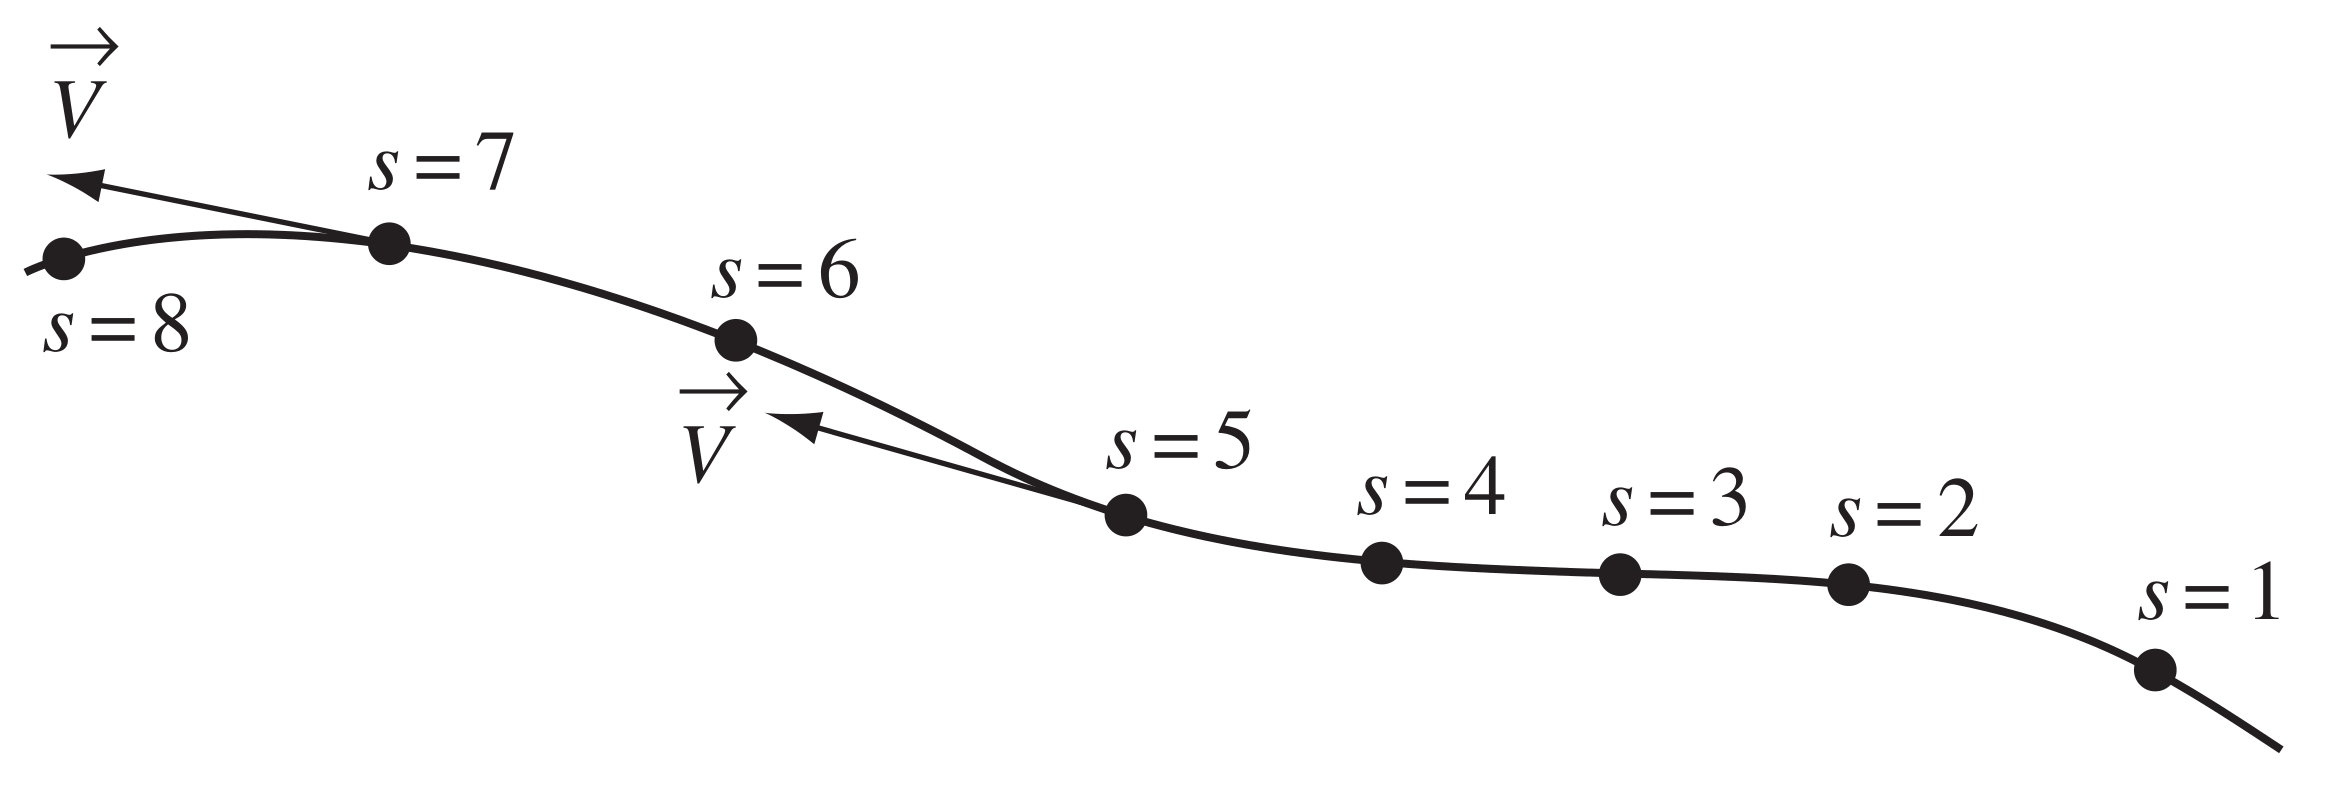
\includegraphics[width=0.6\textwidth]{fig5.4.png}
    \figcaption{\textit{一条曲线,曲线的参数,以及曲线的切向量}}
    \label{fig5.4}
}

注意$s$在坐标变换下不变(它的定义和坐标系无关),而$\vec{V}$的分量变化,因此根据链式法则可得
\begin{equation}
    \begin{pmatrix}
        \rd \xi / \rd s \\
        \rd \eta / \rd s
    \end{pmatrix}
    =
    \begin{pmatrix}
        \partial \xi / \partial x & \partial \xi / \partial y \\
        \partial \eta / \partial x & \partial \eta / \partial y
    \end{pmatrix}
    \begin{pmatrix}
        \rd x / \rd s \\
        \rd y / \rd s
    \end{pmatrix}.
\label{equ5.20}
\end{equation}
这与前面的向量变换律\eqref{equ5.7}式相同。

总结一下现代观点,向量是与某条曲线相切、将$\trd \phi$映射为$\rd \phi / \rd s$的线性函数。这样,下面就能更进一步地研究极坐标系。

\subsection*{极坐标系的1形式基与向量基}
显然,坐标基向量的变换规律为:
\begin{equation*}
    \vec{e}_{\alpha'} = \Lambda\indices{^\beta_{\alpha'}} \vec{e}_\beta,
\end{equation*}
在极坐标下:
\begin{align}
    \vec{e}_r &= \Lambda\indices{^x_r} \Ve_x + \Lambda\indices{^y_r} \Ve_y \label{equ5.21} \\
    &= \frac{\partial x}{\partial r} \Ve_x + \frac{\partial y}{\partial r} \Ve_y \notag \\
    &= \cos \theta \Ve_x + \sin \theta \Ve_y, \label{equ5.22}
\end{align}
类似有
\begin{align}
    \Ve_\theta &= \frac{\partial x}{\partial \theta} \Ve_x + \frac{\partial y}{\partial \theta} \Ve_y \notag \\
    &= -r \sin \theta \Ve_x + r \cos \theta \Ve_y, \label{equ5.23}
\end{align}
注意,上式已经利用了
\begin{equation}
    \Lambda\indices{^x_r} = \frac{\partial x}{\partial r}.
\label{equ5.24}
\end{equation}
类似地,“反向”变换的矩阵元为
\begin{equation}
    \Lambda\indices{^r_x} = \frac{\partial r}{\partial x}.
\label{equ5.25}
\end{equation}
这个变换矩阵十分简单:矩阵指标的上下顺序对应到求导的上下关系就好了。

1形式基的关系可类似求出:
\begin{align}
    \trd \theta &= \frac{\partial \theta}{\partial x} \trd x + \frac{\partial \theta}{\partial y} \trd y, \notag \\
    &= -\frac{1}{r} \sin \theta \trd x + \frac{1}{r} \cos \theta \trd y. \label{equ5.26}
\end{align}
(注意上式与普通的微积分运算\eqref{equ5.4}式相似)。同样可得
\begin{equation}
    \trd r = \cos \theta \trd x + \sin \theta \trd y.
\label{equ5.27}
\end{equation}
根据以上内容可以画出不同点的基(图\ref{fig5.5})。容易画出基向量,1形式基可以画出$\trd r$和$\trd \theta$的等$r$、等$\theta$面辅助进行,不同位置的面的指向不同。

{
    \centering
    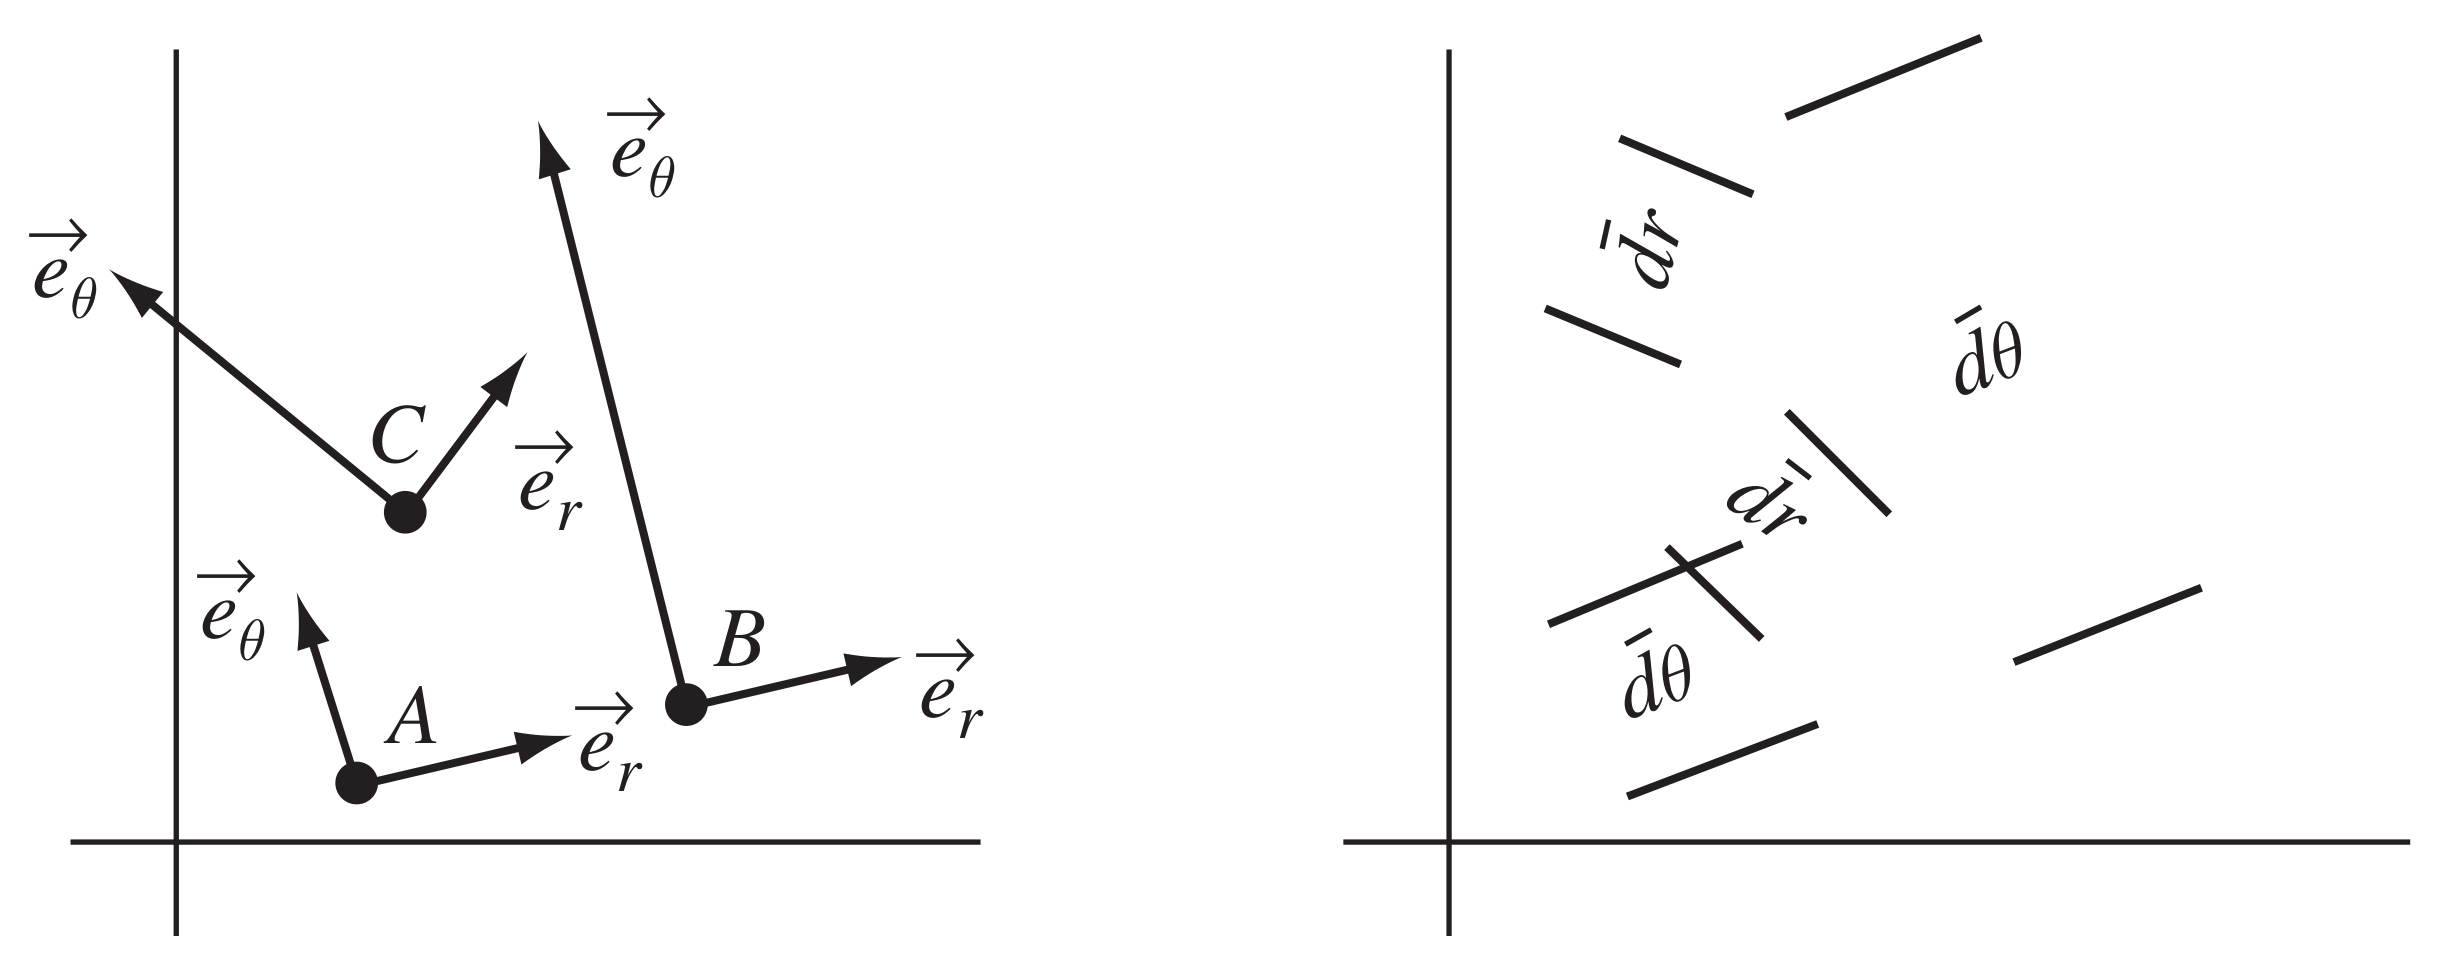
\includegraphics[width=0.7\textwidth]{fig5.5.png}
    \figcaption{极坐标系的向量基与1形式基图示}
    \label{fig5.5}
}

上面体现了一个非常重要的事实:各点的基互不相同。例如,图\ref{fig5.5}中$A$点与$C$点的向量基不平行。这是由于基向量指向坐标增加的方向,而这个方向随着点的改变而改变。此外,基的长度也不是恒定不变的。例如,根据\eqref{equ5.23}式可得

\begin{subequations}
\begin{alignat}{2}
    |\Ve_\theta|^2 &= \Ve_\theta \cdot \Ve_\theta = r^2 \sin^2 \theta + r^2 \cos^2 \theta = r^2,&& \label{equ5.28a} \\
    |\Ve_r| &= 1, \quad |\trd r| = 1, \quad |\trd \theta| = r^{-1}. &&\label{equ5.28b}
\end{alignat}
\end{subequations}
距离原点越远,$\Ve_\theta$的模长越大。因为$\Ve_\theta$在$(r, \theta)$系的分量为$(0, 1)$,意味着它表示$\theta$分量的1单位的位移,即1弧度。在半径更大的地方,移动1弧度的长度更大。因此极坐标基并非\textit{单位}基。其它基的模长容易求出。可以发现,$| \trd \theta|$在$r = 0$附近更大(更紧密),因为一个给定的向量在原点附近覆盖的$\theta$范围更大。

\subsection*{度规张量}
上面的点乘结果都是根据直角坐标系$x, y$中已知的度规来计算的:
\[
    \vec{e}_x \cdot \vec{e}_x = \vec{e}_y \cdot \vec{e}_y = 1, \quad \vec{e}_x \cdot \vec{e}_y = 0;
\]
或者用张量记号写为
\begin{equation}
    \mathbf{g} (\vec{e}_\alpha, \vec{e}_\beta) = \delta_{\alpha \beta} \quad \text{在直角坐标系中。}
\label{equ5.29}
\end{equation}
$\mathbf{g}$在极坐标系的分量是什么?根据分量的定义:
\begin{equation}
    g_{\alpha' \beta'} = \mathbf{g} (\vec{e}_{\alpha'}, \vec{e}_{\beta'}) = \vec{e}_{\alpha'} \cdot \vec{e}_{\beta'},
\label{equ5.30}
\end{equation}
或者根据\eqref{equ5.28}、\eqref{equ5.22}和\eqref{equ5.23}式可得
\begin{equation}
    g_{rr} = 1, \quad g_{\theta \theta} = r^2, \quad  g_{r \theta} = 0. \label{equ5.31}
\end{equation}
由此可得$\mathbf{g}$在极坐标系的分量为
\begin{equation}
    (g_{\alpha \beta})_{\text{polar}} = 
        \begin{pmatrix}
            1 & 0 \\
            0 & r^2
        \end{pmatrix},
\label{equ5.32}
\end{equation}
线元(line element)可以方便地同时表示$\mathbf{g}$的分量以及坐标,线元即为任意“无穷小”位移$\rd \vec{\ell}$的模:
\begin{shaded}
\begin{align}
    \rd \vec{\ell} \cdot \rd \vec{\ell} &= \rd s^2 = |\rd r \vec{e}_r + \rd \theta \vec{e}_\theta |^2 \notag \\
    &= \rd r^2 + r^2 \rd \theta^2. \label{equ5.33}
\end{align}
\end{shaded}
\textit{不要}将这里的$\rd r, \rd \theta$与1形式基$\trd r, \trd \theta$混淆,前者是$\rd \vec{\ell}$在极坐标系的分量,“$\rd$”就是“无穷小$\Delta$”的意思。 

另外有一种导出\eqref{equ5.33}式的方法值得一提。回顾\eqref{equ3.26}式,它表明任何$\binom{0}{2}$张量可以表示为$\binom{0}{2}$张量基$\trd x^\alpha \otimes \trd x^\beta$的线性组合:
\[
    \mathbf{g} = g_{\alpha \beta} \trd x^\alpha \otimes \trd x^\beta = \trd r \otimes \trd r + r^2 \trd \theta \otimes \trd \theta.
\]
尽管上式看起来像\eqref{equ5.33}式,但它们不一样:上式各项是算符,作用于向量$\rd \vec{\ell}$(其分量为$\rd r, \rd \theta$)之后得到\eqref{equ5.33}式。由于相应学科的符号混乱,导致上面两个式子非常不幸地十分相像。大多数教材与论文仍采用“旧式的”表达式——方程\eqref{equ5.33}来表示度规分量,本书遵从这一习惯。

度规分量矩阵存在逆矩阵:
\begin{equation}
    {\begin{pmatrix}
        1 & 0 \\
        0 & r^2
    \end{pmatrix} }^{-1} = 
    \begin{pmatrix}
        1 & 0 \\
        0 & r^{-2}
    \end{pmatrix}.
\label{equ5.34}
\end{equation}
由此可得$g^{rr} = 1, g^{r\theta} = 0, g^{\theta \theta} = 1/r^2$。这可以建立1形式与向量之间的映射。例如,向量场$\phi$的梯度场为$\trd \phi$,则这个1形式相应的向量$\rd \phi$具有分量
\begin{equation}
    (\vec{\rd} \phi)^\alpha = g^{\alpha \beta} \phi_{, \beta}
\label{equ5.35}
\end{equation}
或者写为
\begin{subequations}
\begin{alignat}{2}
    (\vec{\rd} \phi)^r &= g^{r \beta} \phi_{, \beta} = g^{rr} \phi_{, r} + g^{r \theta} \phi_{, \theta} \notag &&   \\
    &= \frac{\partial \phi}{\partial r}. &&\label{equ5.36a} \\
    (\vec{\rd} \phi)^\theta &= g^{\theta r} \phi_{, r} + g^{\theta \theta} \phi_{, \theta} && \notag \\
    &= \frac{1}{r^2} \frac{\partial \phi}{\partial \theta}. && \label{equ5.36b}
\end{alignat}
\end{subequations}
可见,1形式的分量是$(\phi_{, r}, \phi_{, \theta})$,而相应向量的分量是$(\phi_{, r}, \phi_{, \theta} / r^2)$。就算是在欧几里得空间,向量与相应的1形式的分量一般也不相同。直角坐标系是它们在其中唯一相等的坐标系。



\section{极坐标系的张量微积分}
\label{sec5.3}